\chapter{Thảo luận}\label{chapter-5-discussion}

\section{Vì sao teacher-first thắng khi cân bằng compute}\label{why-teacher-first-wins-now-compute-fair}

Cơ chế nền vẫn nhất quán: trên các bài khó, unconditioned student policy hiếm khi sinh được một attempt đúng theo kiểu on-policy, khiến baseline student-first thiếu các quỹ đạo chất lượng cao để distill. Ngược lại, tổ chức teacher-first tiêm vào các quỹ đạo đúng được sinh dưới sự dẫn dắt của execution feedback.

Mở rộng chính mà nghiên cứu đầy đủ này thiết lập là lợi thế đó vẫn sống sót dưới một khung đánh giá compute-matched (§4.4). Ngay cả khi baseline student-first được cấp một ngân sách generation bằng nhau (mười generation mỗi bước), hiệu năng của nó có cải thiện nhưng vẫn kém phương pháp đề xuất. Compute-to-correct frontier còn cho thấy teacher-first đạt các xác suất discovery mục tiêu với tổng số generation ít hơn đáng kể. Điều này đưa tuyên bố cốt lõi của khóa luận từ một lợi thế chỉ-ở-kết-quả sang một lợi thế compute-fair.

\section{Ranh giới value-versus-procedure}\label{the-value-versus-procedure-boundary-validated}

Đánh giá pipeline trên hai miền khác nhau (LiveCodeBench v6 cho code và AIME 2026 cho toán), với cùng một mô hình Qwen3-4B ở cả hai, chỉ ra một ranh giới value-versus-procedure: sự thoát khỏi flat-reward trap xuất hiện khi privileged context mã hóa một \emph{phương pháp} trong tầm với, chứ không khi nó chỉ mã hóa một \emph{giá trị} tĩnh. Việc giữ cố định mô hình làm nổi bật loại reference như một biến tác động chính, dù khoảng cách ngân sách (budget) vẫn là một confounder. Dù vậy, vì phía toán chỉ dựa trên một pilot nhỏ (n = 2), tương phản này được đọc theo hướng \emph{directional} chứ chưa phải kết luận chắc chắn.

\begin{figure}[htbp]
\centering
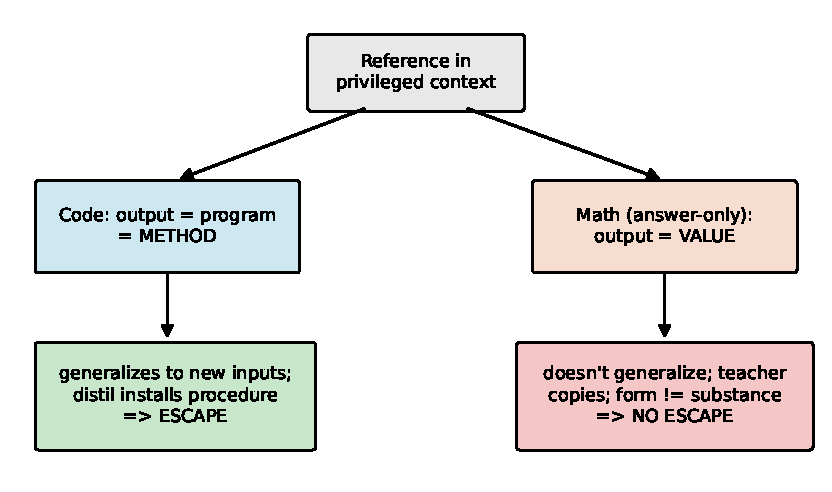
\includegraphics[width=0.9\linewidth]{../figures/bc_fig5_boundary.pdf}
\caption{Ranh giới value-versus-procedure. Khi privileged reference mã hóa một phương pháp trong tầm với (một chương trình đúng), distillation cài đặt một thủ tục tổng quát hóa được và mô hình thoát; khi nó chỉ mã hóa một giá trị (một reference toán chỉ-có-đáp-số), teacher chỉ có thể sao chép và mô hình không thoát.}
\label{fig:bc-boundary}
\end{figure}

Trong miền lập trình, output của mô hình về bản chất là một thủ tục, một chương trình hàm tổng quát hóa được sang các test instance chưa thấy. Execution feedback (lỗi biên dịch, output thời gian chạy, và các metric đánh giá nhiều test case) cung cấp một tín hiệu học phong phú, nhiều chiều, cho phép teacher policy định vị và sửa các lỗi thuật toán. Ngược lại, feedback toán học từ pilot AIME bị giới hạn nghiêm ngặt ở một giá trị số tĩnh, không có bất kỳ suy dẫn từng bước nào.

Khi mô hình gốc không tự khám phá được lời giải đúng, feedback chỉ-có-giá-trị này ép teacher vào một copy-regime nông cạn. Vì reference không chứa thủ tục hay lập luận nền nào, quá trình self-distillation đứng yên, để lại student kẹt ở mức 0. Trên pilot nhỏ này, do đó, context giàu thông tin dường như suy biến thành sao chép đáp án trừ khi nó mang một phương pháp cấu trúc mà student có thể nội hóa.

\section{Sự đè nén epistemic, và ý nghĩa của nó ở đây}\label{epistemic-suppression-and-what-it-means-here}

Việc đưa reasoning trace vào miền code (§4.7) cho phép nghiên cứu này kết nối trực tiếp với khung của Kim và cộng sự {[}2{]}. Kết quả chỉ ra rằng distill từ một context giàu thông tin, feedback-conditioned làm giảm các epistemic marker (ví dụ các token biểu thị bất định, các tín hiệu tự sửa), và hiệu ứng này tích lũy qua các bước tối ưu tại thời điểm suy luận nối tiếp nhau.

Nghiên cứu bổ sung một điều kiện phụ thuộc regime cho phê phán về epistemic suppression, được trình bày như một cách diễn giải chứ không phải một cơ chế đã chứng minh. Trong miền code, nơi privileged reference là một chương trình hợp lệ về cấu trúc, sự đè nén ở mức token \emph{đồng xảy ra} (co-occur) với việc functional correctness cải thiện. Vì correctness được đo trên held-out test, mức tăng phản ánh một phương pháp tổng quát hóa được chứ không phải một đáp án được chép; cách đọc tự nhiên là cả sự đè nén lẫn mức tăng correctness đều là hệ quả của việc củng cố một thủ tục đúng, chứ không phải sự đè nén gây ra mức tăng. Như Kim và cộng sự {[}2{]} đã chỉ ra, trong math leak regime, cùng một sự đè nén bề mặt lại nhất quán với việc sao chép đáp án, bởi reference chỉ là một giá trị trơ, không có thủ tục nào để nội hóa. Theo cách đọc này, đè nén không mặc nhiên có hại; ý nghĩa của nó phụ thuộc vào việc privileged context mang một phương pháp tái lập được hay một giá trị thô. Để cô lập loại reference như nguyên nhân tác động, cần một ablation cùng-miền (một reference chỉ-có-giá-trị so với một reference mang-phương-pháp trên code), điều này được để cho hướng phát triển sau.

\section{Vị trí so với bài báo gốc}\label{position-relative-to-the-parent-paper}

Công trình này được định vị đối chiếu với formulation của Hübotter và cộng sự {[}1{]}. Chúng tôi trình bày một tổ chức teacher-first của execution-guided self-distillation, tăng tốc test-time discovery dưới một giao thức đánh giá compute-fair. Cùng với việc đo hành vi epistemic trong tối ưu code và việc đặc trưng hóa ranh giới value-versus-procedure, nó giải quyết một số câu hỏi vận hành mà bài báo gốc để ngỏ.
